\subsection{Addressing programs with Conditionals}
        We first consider programs with conditionals. The following two properties holds for any candidates of programs having conditional branching. 

        \begin{property}{Candidates of Programs with Conditionals}
            \label{CondB1}
            Let $B1$ be the sets of events based on a branch of a conditional in a program $P$. Let $C$ be any Candidate of $P$, Consider $b1$ to be representative of any event in $B1$ and an event $k$ outside the conditional branch. Then:
            \begin{align*}
                \exists C \in P \ \text{s.t.} b1 \notin C  
            \end{align*}
            There exists a candidate of the program such that events from the branch cannot be part of it\footnotemark. 
        \end{property}

        The above property is general for conditionals, being 1-branch or 2-branch. The latter however, has another property which we define below:

        \begin{property}{Candidates of Programs with Conditionals (2-branch)}
            \label{CondB2}
            Let $B1,B2$ be two sets of events based on each branch of a conditional in a program $P$. Let $C$ be any Candidate of $P$,  Consider $b1,b2$ to be representative of any event in $B1,B2$ respectively. Then:
            \begin{align*}
                \nexists C \in P \ \text{s.t.} \ b1 \in C \ \wedge \ b2 \in C \\ 
            \end{align*}
            There cannot exist any candidate of the program such that events from both sets can be part of it. 
        \end{property}

        The figure below summarizes the two forms of conditionals we can have in any program. 
        \begin{figure}[H]
            \centering 
            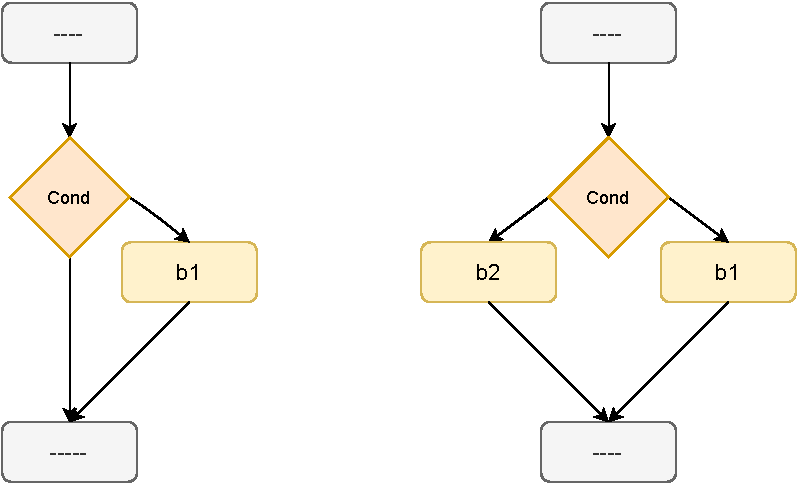
\includegraphics[scale=0.7]{5.InstructionReordering/5.ValidReorderingProgram/Conditionals2Form.pdf}
            \caption{Two forms of conditonals}
        \end{figure}

        \footnotetext{While the property for 1 branch may not always hold (it can be the case that the branch is always taken in any execution) we are defining it for any program.}

        \begin{corollary}
            \label{ReordCond}
            Consider a program $P$ and its candidates $C_1, C_2, ... , C_n$ in which events $e$ and $d$ present in all of them with $\reln{e}{ao}{d}$. Consider the set of corresponding candidates $C'_1, C'_2, ... , C'_n$ after reordering $e$ and $d$ and its corresponding program $P'$. If the following two conditions hold:
            \begin{gather*}
                Reord(e,d) \ \wedge \ 
                ( \forall C_{i \in [1,n]}, \forall k \in C_i \ \text{s.t.} \ \reln{e}{ao}{k} \wedge \reln{k}{ao}{d}, \    
                Reord(e,k) \wedge Reord(k,d) ) \\
                \nexists C \in P \ s.t. \ 
                    (e \in C \ \wedge \ d \notin C) \ \vee \ 
                    (e \notin C \ \wedge \ d \in C) 
            \end{gather*}
            then the set of observable behaviors of $P'$ is a subset of that of $P$. 
        \end{corollary}

        \begin{proof}
        
            We prove the second condition first. 
            Suppose the second condition does not hold. Thus we would have
            \begin{align*}
                \exists C \in P \ s.t. \ 
                (e \in C \ \wedge \ d \notin C) \ \vee \ 
                (e \notin C \ \wedge \ d \in C)
            \end{align*}

            This can only happen, if events $e$ or $d$ are part of a conditional branch.
            \begin{itemize}
                \item C1: Both $e$ and $d$ are part of conditional branches

                    If $e$ and $d$ are in different branches of same conditonal, then by Prop \ref{CondB2}, we would have 
                    \begin{align*}
                        \nexists C \in P \ \text{s.t.} \ e \in C \ \wedge \ d \in C 
                    \end{align*}
                    But our Corollary assumption is that there exists such candidates. Hence, this cannot be the case.

                    If $e$ and $d$ are of the same conditonal branch, and neither one of them belong in any conditional branch nested within, then our assumption does not hold. 

                    \begin{figure}[H]
                        \centering 
                        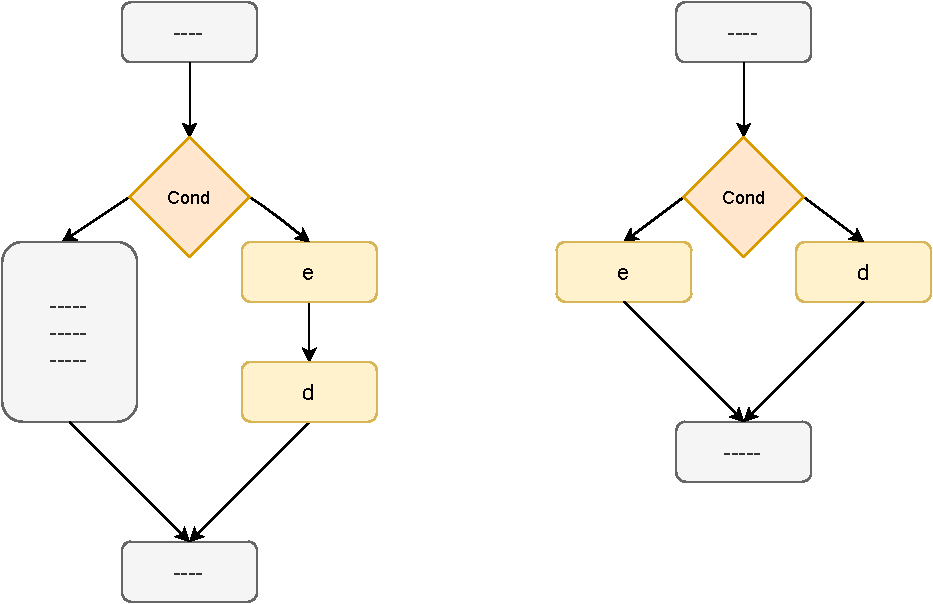
\includegraphics[scale=0.5]{5.InstructionReordering/5.ValidReorderingProgram/ConditionalsProofFig1.pdf}
                        \caption{The above two cases where our assumption does not hold.}
                    \end{figure}

                    If $e$ and $d$ belong to branches of differnt conditionals, then they can be of two forms, viz. where one conditional branch is nested within the other or both conditonal branches are not nested within each other.  

                    \begin{figure}[H]
                        \centering 
                        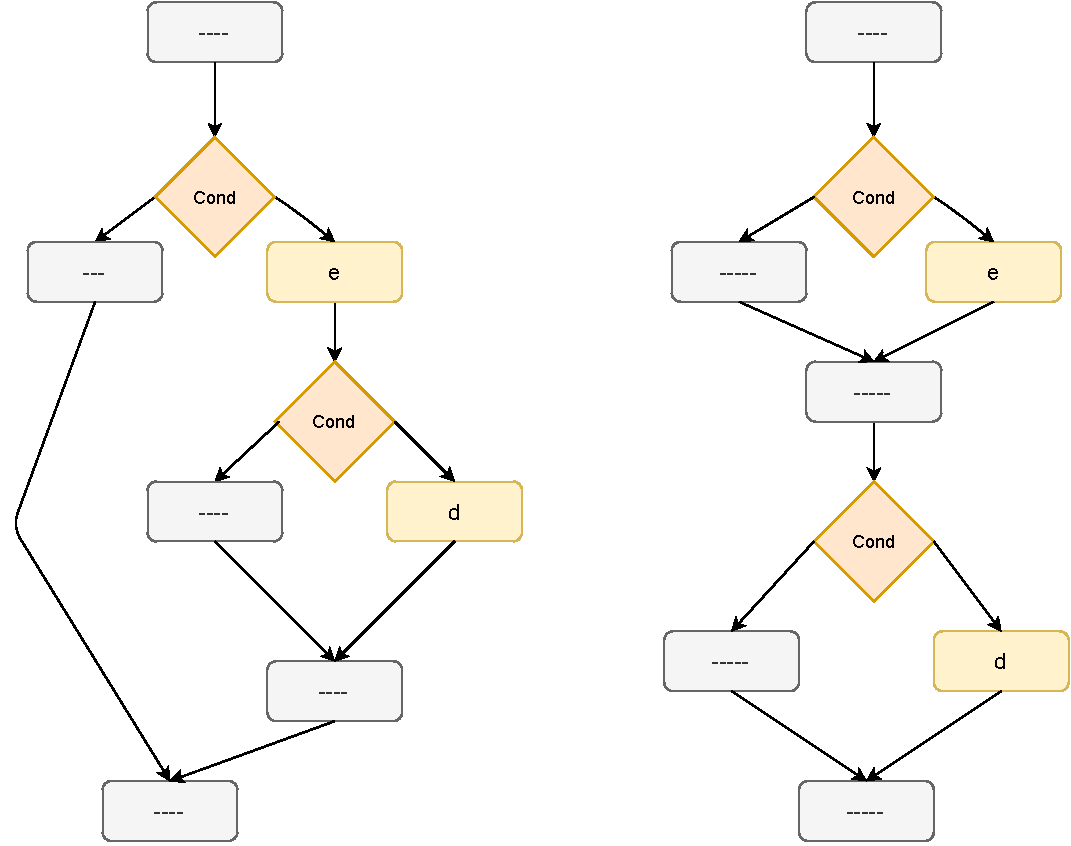
\includegraphics[scale=0.5]{5.InstructionReordering/5.ValidReorderingProgram/ConditionalsProofFig2.pdf}
                        \caption{Two cases where $e$ and $d$ can both be part of some conditional.}
                    \end{figure}

                    For the first form, without loss of generality, let us consider $d$ is part of conditional branch nested within $e$'s branch. 

                    By Prop \ref{CondB2}, there would exist some event $l$ in another branch such that 
                    \begin{align*}
                        \nexists C \in P \ \text{s.t.} \ d \in C \ \wedge \ l \in C 
                    \end{align*}
                    On reodering $e$ and $d$, we have 
                    \begin{align*}
                        \nexists C \in P' \ \text{s.t.} \ e \in C \ \wedge \ l \in C 
                    \end{align*}
                    Thus we have 
                    \begin{align*}
                        \exists C \in P' \ \text{s.t} \ d \in C \ \wedge \ l \in C
                    \end{align*}
                    giving us a new Candidate in $P'$ not in $P$. 
                    Irrespective of $d$ being a read or a write, there could be a new $\stck{_{rf}}$ relation be formed with some event$k$. Thus, we have a new observable behavior. 

                    By Prop \ref{CondB1}, we would have 
                    \begin{align*}
                        \exists C \in P \ \text{s.t.} \ d \notin C  
                    \end{align*}
                    Suppose there exists another event $l$ in the same branch as $d$, but not part of any nested conditional within. Then we also have 
                    \begin{align*}
                        \nexists C \in P \ \text{s.t.} \ 
                        (d \in C \ \wedge \ l \notin C) 
                        \ \vee \ 
                        (d \notin C \ \wedge \ l \in C)   
                    \end{align*}

                    \critic{red}{The above conclusion need not be proved. Neither should it be put as a property.}

                    On reodering $e$ and $d$, we have by Prop \ref{CondB1}
                    \begin{align*}
                        \exists C \in P' \ \text{s.t.} \ e \notin C  
                    \end{align*}
                    We also have that 
                    \begin{align*}
                        \exists C \in P' \ \text{s.t} \ (d \notin C \ \wedge \ l \in C) 
                    \end{align*}
                    giving us a new Candidate in $P'$ not in $P$.
                    Irrespective of $d$ being a read or a write, there could be a new $\stck{_{rf}}$ relation be formed with some event$k$. Thus, we have a new observable behavior. 

                    For the second case, suppose they are part of conditonals of typr Prop \ref{CondB2}. Therefore, there exists events $l1, l2$ in their respective counter branches such that:
                    \begin{align*}
                        \nexists C \in P \ \text{s.t.} \ e \in C \wedge l1 \in C \\ 
                        \nexists C \in P \ \text{s.t.} \ d \in C \wedge l2 \in C 
                    \end{align*} 
                    Reodering $e$ and $d$ would result in program $P'$ such that
                    \begin{align*}
                        \nexists C' \in P' \ \text{s.t.} \ d \in C \wedge l1 \in C \\ 
                        \nexists C' \in P' \ \text{s.t.} \ e \in C \wedge l2 \in C  
                    \end{align*}  
                    Thus giving us new Candidates in $P'$ not in $P$ such that 
                    \begin{align*}
                        e \in C' \wedge l1 \in C' \\ 
                        d \in C' \wedge l2 \in C'
                    \end{align*}
                    Irrespective of $e$ and $d$ being reads or writes, there could be a new $\stck{_{rf}}$ relation be formed with some event$k$. Thus, we have a new observable behavior. 

                    From the above we can also conclude that even if $e$ or $d$ (one of them) are in a conditional branch satsifying Prop \ref{CondB2}, a new observable behavior can be introduced due to a new Candidate that violates the original Prop \ref{CondB2} of every candidate of program $P$.

                    Lastly, suppose both $e$ and $d$ are part of conditonal branches satisfying Prop \ref{CondB1}, then we have 
                    \begin{align*}
                        \exists C \in P \ \text{s.t.} \ e \notin C \\
                        \exists C \in P \ \text{s.t.} \ d \notin C
                    \end{align*}
                    Let $B_e$ and $B_d$ be the respective set of events that belong in the same branch as $B_e$ and $B_d$ respectively. Thus, by Prop \ref{CondB1}, we also have 
                    \begin{align*}
                        e \notin C \ \Rightarrow \ \nexists k \in B_e \ \text{s.t.} \ k \in C \\
                        d \notin C \ \Rightarrow \ \nexists k \in B_d \ \text{s.t.} \ k \in C
                    \end{align*}
                    Now after reordering $e$ and $d$, we could have a Candidate in $P'$ such that the above conditions are violated. Irrespective of $e$ and $d$ being reads or writes, there could be a new $\stck{_{rf}}$ relation be formed with some event$k$. Thus, we have a new observable behavior\footnotemark.  

                    \footnotetext{One may think of it as introducing a new event in a Candidate, thus causing new observable behavior.}

                \item C2: Without loss of generality, let us consider $d$ is part of conditional branch but $e$ is not. 
                
                    By Prop \ref{CondB2}, there would exist some event $l$ in another branch such that 
                    \begin{align*}
                        \nexists C \in P \ \text{s.t.} \ d \in C \ \wedge \ l \in C 
                    \end{align*}
                    On reodering $e$ and $d$, we have 
                    \begin{align*}
                        \nexists C \in P' \ \text{s.t.} \ e \in C \ \wedge \ l \in C 
                    \end{align*}
                    Thus we have 
                    \begin{align*}
                        \exists C \in P' \ \text{s.t} \ d \in C \ \wedge \ l \in C
                    \end{align*}
                    giving us a new Candidate in $P'$ not in $P$. 
                    Irrespective of $e$ being a read or a write, there could be a new $\stck{_{rf}}$ relation be formed with some event$k$. Thus, we have a new observable behavior. 

                    By Prop \ref{CondB1}, we would have 
                    \begin{align*}
                        \exists C \in P \ \text{s.t.} \ d \notin C  
                    \end{align*}
                    On reodering $e$ and $d$, we have 
                    \begin{align*}
                        \exists C \in P' \ \text{s.t.} \ e \notin C  
                    \end{align*}
                    Thus we have 
                    \begin{align*}
                        \nexists C \in P' \ \text{s.t} \ d \notin C 
                    \end{align*}
                    giving us a new Candidate in $P'$ not in $P$.
                    Irrespective of $e$ being a read or a write, there could be a new $\stck{_{rf}}$ relation be formed with some event$k$. Thus, we have a new observable behavior. 

                    \begin{figure}[H]
                        \centering 
                        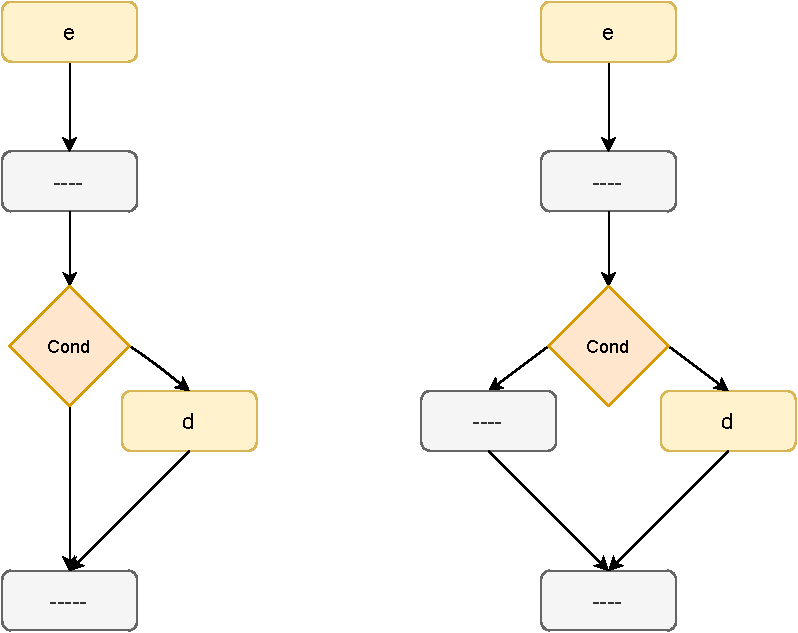
\includegraphics[scale=0.5]{5.InstructionReordering/5.ValidReorderingProgram/ConditionalsProofFig3.pdf}
                        \caption{Two cases where only $d$ is a part of some conditional branch.}
                    \end{figure}

            \end{itemize}

            Now that we have that the second condition must hold, we prove the first condition too must hold. Let $C_i$ and $C_i'$ be the candidates before and after reordering $e$ and $d$. From the first condition we have then for $C_i$
            \begin{align*}
                \forall \ k \ \textit{s.t.} \ 
                \reln{e}{ao}{k} \ \wedge \ \reln{k}{ao}{d} \ . \ 
                Reord(e,k) \ \wedge \ Reord(k,d).
            \end{align*}
            The above is Corollary 1 (tag properly), thus giving us that the observable behaviors of $C_i'$ is a subset of $C_i$. By property of unions of sets, we can conclude that the set of Observable Behaviors of $P'$ is a subset of that of $P$.

        \end{proof}

%------------------------------------------------------------------------------------------------------------------------------------------

        In addition to the above proof, we also show certain counter examples where reordering may not be safe to do. This faciliates better understanding of the proof and its arguments. These counter examples are with respect to reordering of writes. 

        \critic{purple}{While showing reordering of reads, one must note that the introduction of new observable behaviors is dependant on the fact that a candidate execution has a local variable which must have not been there beacause the conditional branch was not taken. Note that this fact does not rely on the consistency rules of the memory model. It could be the case that the compiler instantiates the local variables to some default value (say 0), and then decides to reorder a read outside a conditional on the assertion that the read of local variable will return the same constant value. Having such an assertion in general might not be always certain. (Discuss with Clark)}

        \paragraph{Case when $e$ is not in any conditional branch but $d$ is.}

            \critic{blue}{One example with two branches.}
            The example below shows a case with a conditonal having two branches where reordering $e$ and $d$ is not safe. 
            \begin{figure}[H]
                \centering 
                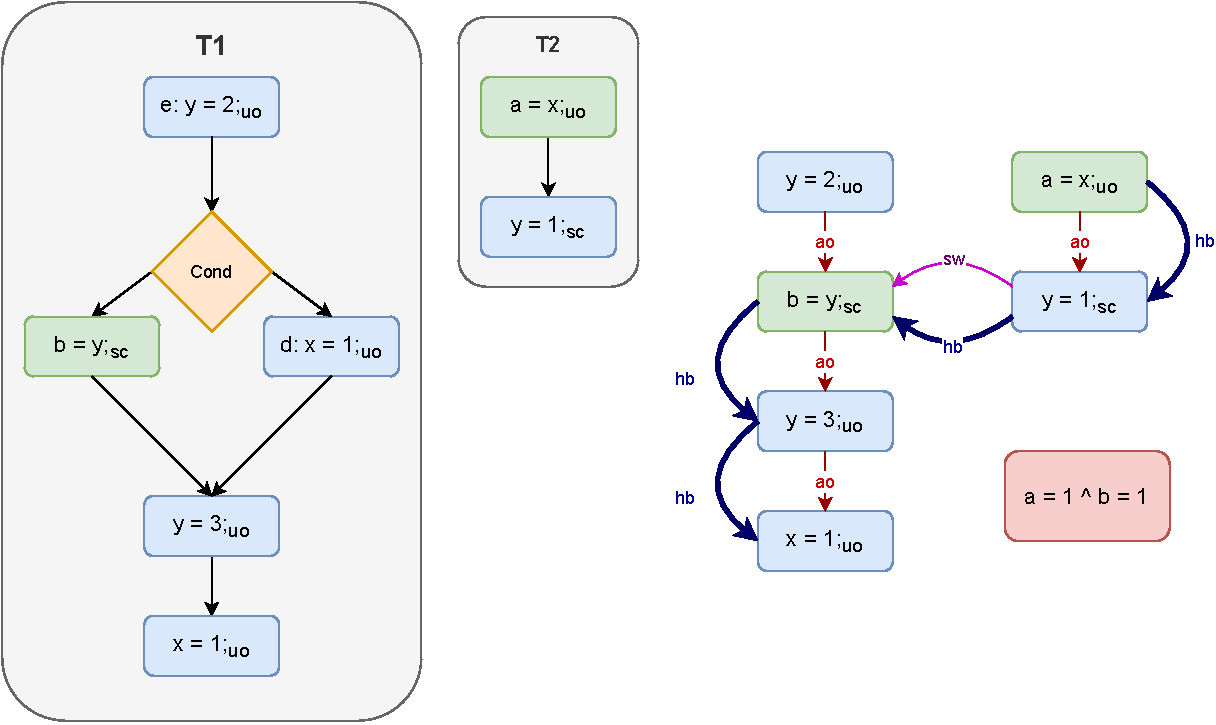
\includegraphics[scale=0.7]{5.InstructionReordering/5.ValidReorderingProgram/CounterExamples1a(Conditionals).pdf}
                \caption{}
            \end{figure}

            The figure on the left above shows an example of such a program.  
            The figure on the right shows the Candidate Execution where the red box outcome is not allowed when the left branch of the conditional is taken.
            \begin{itemize}
                \item From the Candidate Execution, we can infer $\reln{a=x;_{uo}}{hb}{\reln{y=1;_{sc}}{hb}{\reln{b=y;_{sc}}{hb}{\reln{y=3;_{uo}}{hb}{x=1;_{uo}}}}}$.
                \item By Axiom \ref{CoRe}, the read $a$ cannot have value of $x$ read as $1$. 
                \item This inference was due to $\reln{a=x;_{uo}}{hb}{x=1;_{uo}}$.
            \end{itemize}

            \begin{figure}[H]
                \centering 
                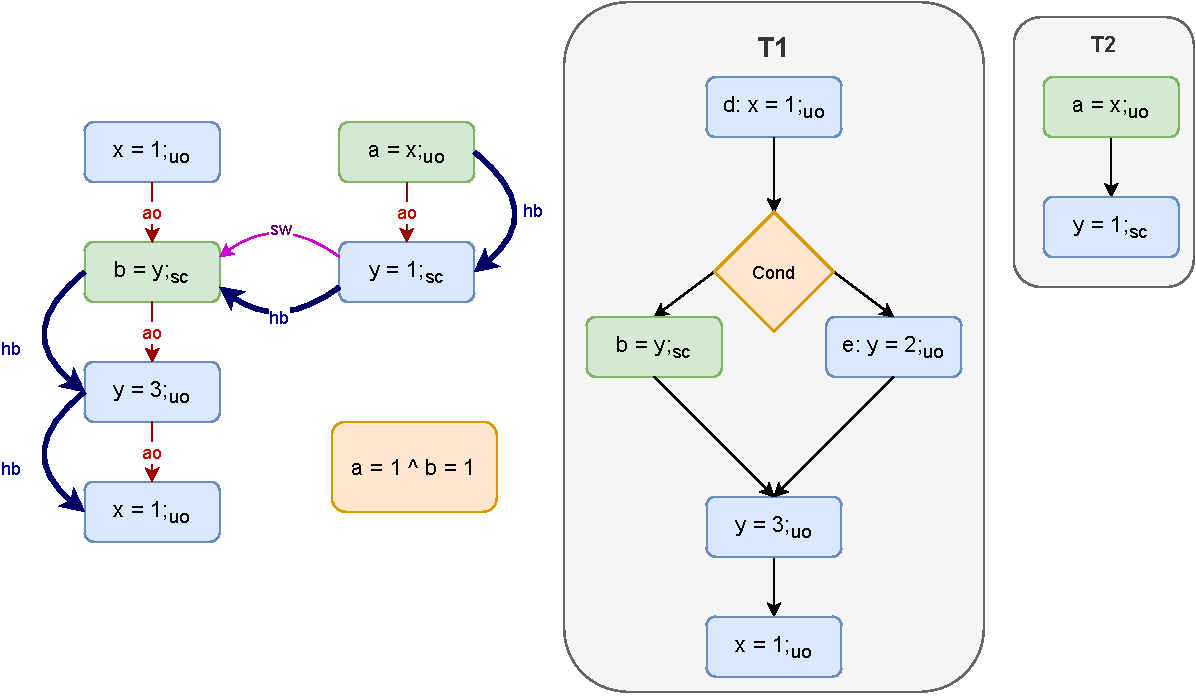
\includegraphics[scale=0.7]{5.InstructionReordering/5.ValidReorderingProgram/CounterExamples1b(Conditionals).pdf}
                \caption{}
            \end{figure}
            The figure on the right above shows the program after reordering $e$ and $d$.  
            The figure on the left shows a Candidate Execution where the yellow box outcome is allowed when the left branch of the conditional is taken.
            \begin{itemize}
                \item From the Candidate Execution, we can infer $\reln{a=x;_{uo}}{hb}{x=1;_{uo}}$. 
                \item But there is no $\stck{_{hb}}$ relation with event $d$ and the read to $x$, i.e. $\neg \reln{a=x;_{uo}}{hb}{d:x=1;_{uo}}$
                \item No Axiom restricts the read $a$ to have value of $x$ as $1$.
            \end{itemize}

            \critic{blue}{One example with one branch.}

            \begin{figure}[H]
                \centering 
                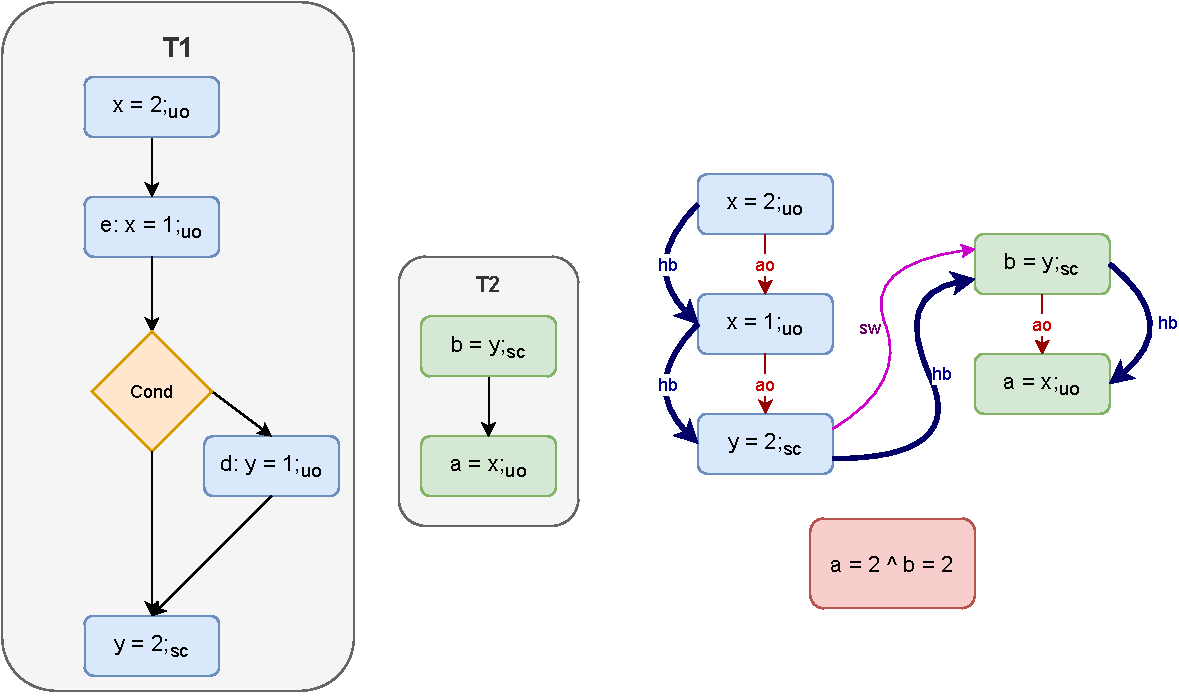
\includegraphics[scale=0.7]{5.InstructionReordering/5.ValidReorderingProgram/CounterExamples2a(Conditionals).pdf}
                \caption{}
            \end{figure}
            The figure on the left above shows an example of such a program.  
            The figure on the right shows the Candidate Execution where the red box outcome is not allowed when the conditional branch is not taken.
            \begin{itemize}
                \item From the Candidate Execution, we can infer $\reln{x=2;_{uo}}{hb}{\reln{x=1;_{uo}}{hb}{\reln{y=2;_{sc}}{hb}{\reln{b=y;_{sc}}{hb}{a=x;_{uo}}}}}$.
                \item By Axiom \ref{CoRe}, the read $a$ cannot have the value of $x$ to be read as $2$.  
                \item This inference was due to the realtion $\reln{x=2;_{uo}}{hb}{\reln{x=1;_{uo}}{hb}{a=x;_{uo}}}$.
            \end{itemize}

            \begin{figure}[H]
                \centering 
                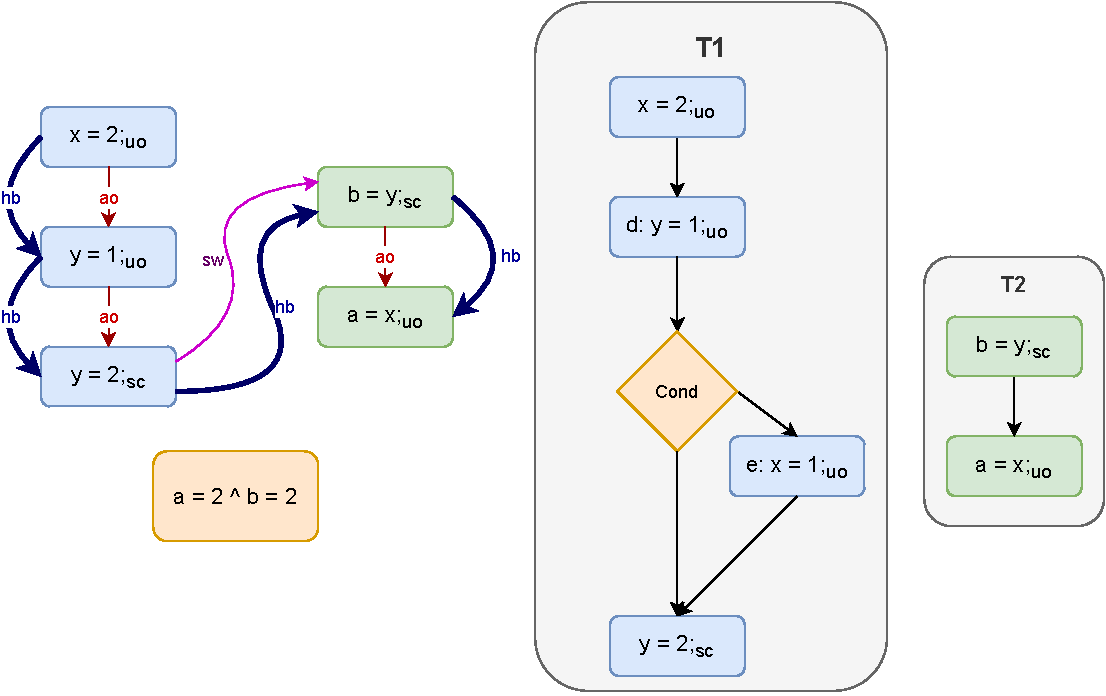
\includegraphics[scale=0.7]{5.InstructionReordering/5.ValidReorderingProgram/CounterExamples2b(Conditionals).pdf}
                \caption{}
            \end{figure}
            The figure on the right above shows the program after reordering $e$ and $d$.  
            The figure on the left shows a Candidate Execution where the yellow box outcome is allowed when the conditional branch is not taken.
            \begin{itemize}
                \item From the Candidate Execution, we can infer $\reln{x=1;_{uo}}{hb}{a=x;_{uo}}$. 
                \item But there is no $\stck{_{hb}}$ relation with event $e$ and the read to $x$, i.e. $\neg \reln{e:x=1;_{uo}}{hb}{a=x;_{uo}}$.
                \item No Axiom restricts the read $a$ to have value of $x$ as $2$.
            \end{itemize}


        \paragraph{Case when $e$ is part of a conditonal branch $B_e$ and $d$ is part of another conditonal branch $B_d$ nested within $B_e$.}

            This case is symmetric to the above. Hence, we do not show another counter example for it. (just consider the code of T1 above to be as a whole under a conditional.)

        \paragraph{Case when $e$ and $d$ are part of different conditional branches. One not nested in the other.}

            \critic{blue}{One example suffices, irrespective of 2 branch or one branch.}

            \begin{figure}[H]
                \centering 
                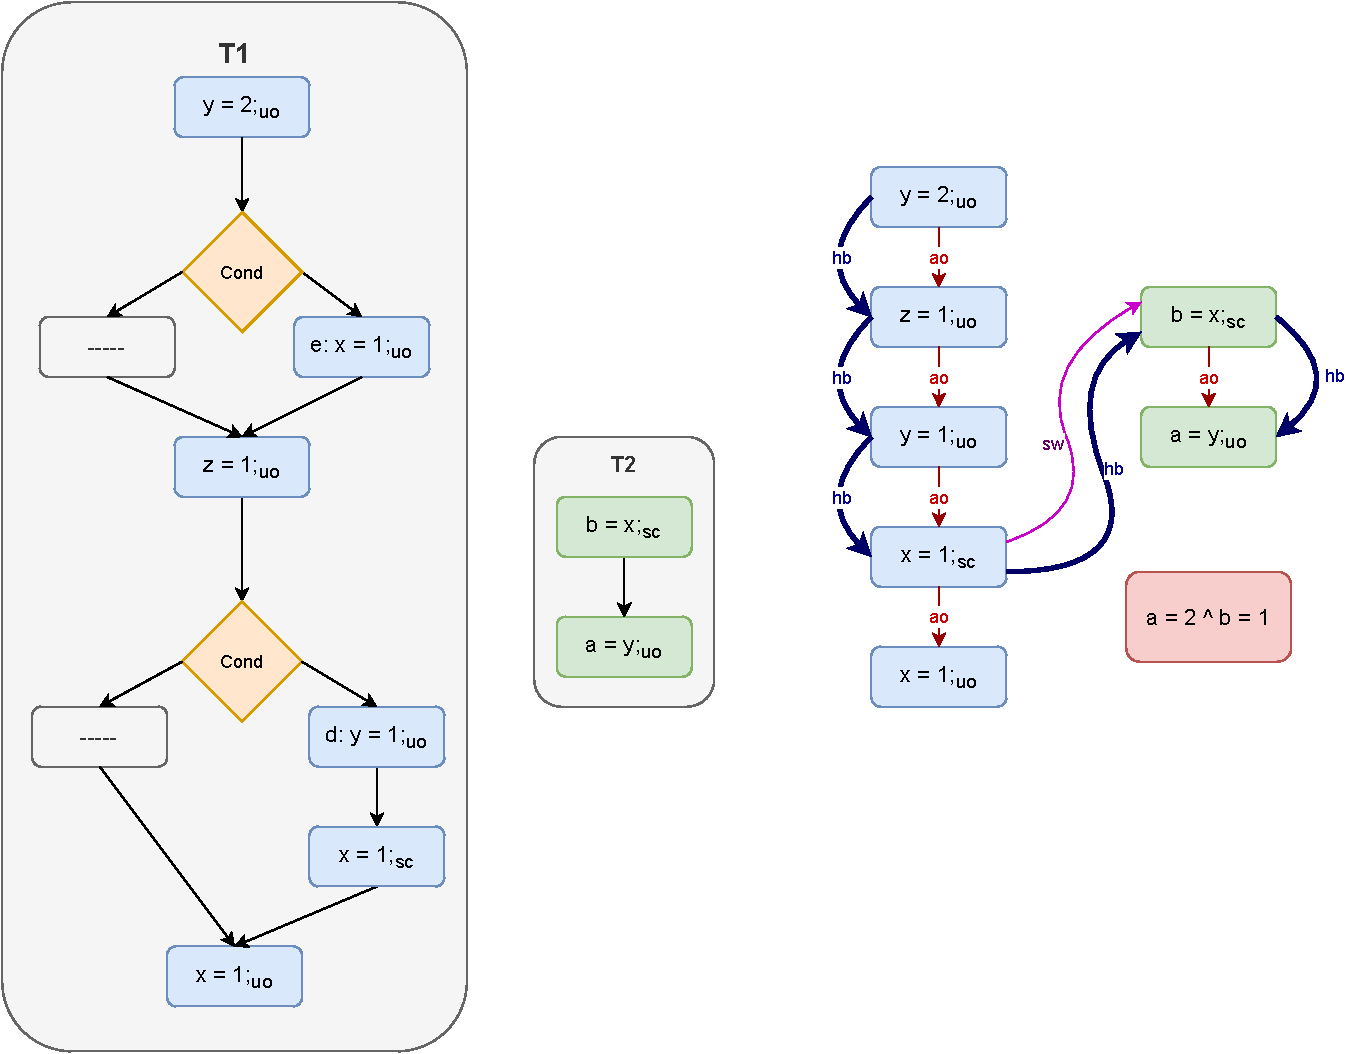
\includegraphics[scale=0.7]{5.InstructionReordering/5.ValidReorderingProgram/CounterExamples3a(Conditionals).pdf}
                \caption{}
            \end{figure}
            The figure on the left above shows an example of such a program.  
            The figure on the right shows the Candidate Execution where the red box outcome is not allowed when the left branch of the first conditional is not taken while the left branch of the second conditional is.
            \begin{itemize}
                \item From the Candidate Execution, we can infer $\reln{y=2;_{uo}}{hb}{\reln{z=1;_{uo}}{hb}{\reln{y=1;_{uo}}{hb}{\reln{x=1;_{sc}}{hb}{\reln{b=x;_{sc}}{hb}{a=y;_{uo}}}}}}$.
                \item By Axiom \ref{CoRe}, the read $a$ to $y$ cannot have the value $2$. 
                \item The above inference is due to the relations $\reln{y=2;_{uo}}{hb}{\reln{y=1;_{uo}}{hb}{a=y;_{uo}}}$.
            \end{itemize}

            \begin{figure}[H]
                \centering 
                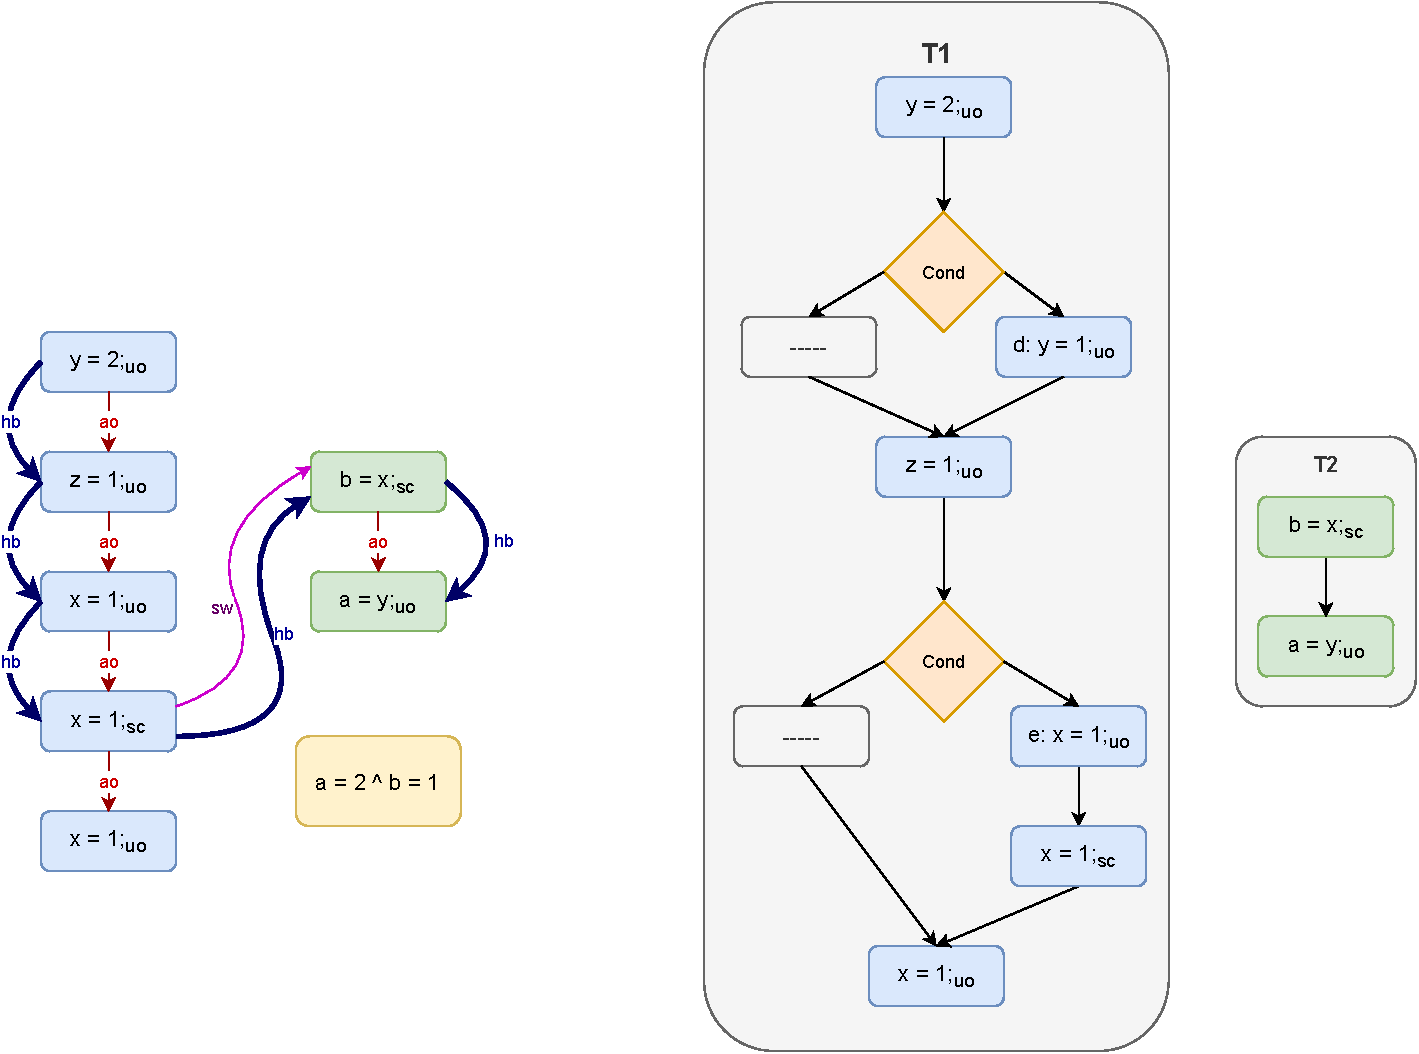
\includegraphics[scale=0.7]{5.InstructionReordering/5.ValidReorderingProgram/CounterExamples3b(Conditionals).pdf}
                \caption{}
            \end{figure}
            The figure on the right above shows the program after reordering $e$ and $d$.  
            The figure on the left shows a Candidate Execution where the yellow box outcome is allowed when the left branch of the first conditional is not taken but that of second conditional is.
            \begin{itemize}
                \item From the Candidate Execution, we can infer $\reln{y=2;_{uo}}{hb}{a=y;_{uo}}$. 
                \item But there is no $\stck{_{hb}}$ relation with event $d$ and the read to $y$, i.e. $\neg \reln{e:y=1;_{uo}}{hb}{a=y;_{uo}}$ and $\neg \reln{y=2;_{uo}}{hb}{y=1;_{uo}}$.
                \item From the above we can infer that no Axiom restricts the read $a$ to have value of $y$ as $2$.
            \end{itemize}

%------------------------------------------------------------------------------------------------------------------------------------------